\documentclass[a4paper]{article}

\usepackage[utf8]{inputenc}
\usepackage{fancyhdr}
\usepackage{geometry}
\usepackage[frenchb]{babel}
\usepackage{libertine}
\usepackage[pdftex]{graphicx}
\usepackage{hyperref}
\usepackage{slashbox}
\usepackage[T1]{fontenc}
\usepackage{multirow}
\usepackage{graphicx}
\usepackage{array,multirow,makecell}
\setcellgapes{1pt}
\makegapedcells
\newcolumntype{R}[1]{>{\raggedleft\arraybackslash }b{#1}}
\newcolumntype{L}[1]{>{\raggedright\arraybackslash }b{#1}}
\newcolumntype{C}[1]{>{\centering\arraybackslash }b{#1}}
\geometry{a4paper}
\geometry{top=3cm, bottom=3cm, left=3.5cm, right=3.5cm}

\begin{document}

\large
\begin{titlepage}
		\title{Rapport de la première soutenance : Lucidity by the Chamallow}
		
		\author{CLAUS Marion -  DELECROIX Thomas - GINANE Charles - MARCHAUD Laurent} 

		
\end{titlepage}


\pagestyle{fancy}
\lhead{The Chamallow}
\rfoot{EPITA Supinfo}
\renewcommand{\footrulewidth}{0.4pt}
\rhead{Rapport de la première soutenance}

 \begin{titlepage}
\centering
\maketitle

\includegraphics[scale=0.3]{Logo.png}

  \end{titlepage}

\tableofcontents 

\newpage

\section{Introduction :}

\quad

Jeudi 28 Janvier 2016, Epita, Villejuif. Notre cahier des charges est validé, après quelques mises au point au sein du groupe, nous nous sommes lancés dans l'univers de Unity. C'est ainsi que le jeu Lucidity vit le jour sur les écrans du groupe The Chamallow, sortant de multiples lignes de code. 
Voici l'heure de vous présenter notre rapport sur l'avancement de notre projet pour notre première soutenance. Celle-ci permettra au jury de découvrir nos premiers pas dans la création d'un jeu vidéo.
Nous rappelons que ce projet va nous permettre de connaître la notion de travail de groupe et de pouvoir enrichir nos connaissances dans le domaine l’informatique mais aussi dans la gestion et l’organisation de tâches entre nous.
Dans ce rapport, nous vous représenterons dans un premier temps notre groupe et notre projet, puis nous verrons l'avancement du projet, ensuite le bilan réalisé par chacun des membres de notre groupe et enfin pour finir notre site web.

Nous vous souhaitons une agréable lecture.

\quad

\quad 


\begin{center}

\textbf{The Chamallow}

\end{center}

\quad

\newpage

\section{Présentation :}

\quad

Bref, trêve de discussion, commençons cette première partie par quelques petits rappels concernant notre projet, ainsi que notre groupe.

\quad

	\subsection{Présentation du groupe:}

\quad

Le groupe “The Chamallow”  est composé de 4 membres, la chance a fait que nous avons aucun redoublement. il est composé de  :

 - Marion “Santa “ CLAUS  qui s’est occupée de la conception du monde en créant la map du premier niveau et aussi du moteur graphique.

 - Thomas “Tetra” DELECROIX notre chef de projet , qui s’est chargé du moteur physique.

 - Charles “Gigi” GINANE qui a géré le gameplay tel que l’HUD (ou l’ATH)  

 - Laurent “aluxima” MARCHAUD qui s’est occupé des sons et principalement du site du projet.


\quad

	\subsection{Présentation du projet:}
\quad

    Le projet Lucidity est un jeu développé sous Unity, ce jeu à la première personne se base sur la réflexion / puzzle et l’interaction avec le décor afin de trouver la solution et d’arriver au terme du niveau. Il se base sur deux jeux plus ou moins connus, tels que “Portal” et “Qube”.
Notre environnement est constitué de salles closes dans lesquelles le joueur doit effectuer une suite d’actions en interaction avec le décor lui permettant de sortir de la salle et de passer à un niveau supérieur. Pour l'interaction avec le décor se fait grâce à la “Lucidité”, la ressource primaire du jeu. Elle est contenable en quantité limitée dans une bouteille spéciale que le joueur transportera dans son dos. Cette ressource peut être récoltée au niveau des sources, rares, présentes qu’à certains endroits de la carte. Une fois que le personnage n’a plus de Lucidité, il doit recommencer à partir du dernier checkpoint.

\quad

\quad



\newpage


\section{La réalisation du projet}

\quad

    Nous allons maintenant vous présenter l’avancée du projet en partant de la validation du cahier des charges, soit le 28 Janvier 2016 jusqu’à la date de la première soutenance

	\subsection{Rappel des objectifs pour la première soutenance:}


    Voici le tableau qui rappelle l’avancement des différentes tâches de notre projet que nous avions prévues dans notre cahier des charges pour la première soutenance.

\quad

\underline{\textbf{Légende de la figure 1:}} : 

\quad
	   -  -     : Pas de participation

 \quad
	- X     : Faible implication

 \quad
	- XX   : Moyenne implication

 \quad
	- XXX : Forte implication 

\quad

\quad 

\begin{tabular}{|c||c|c|c|c|}
\hline Domaine / Nom & Laurent & Charles & Marion & Thomas \\ 
\hline Moteur graphique & - & - & XX & X\\
\hline Moteur physique & - & - & X & XX\\
\hline Site & XXX & X & - & -\\
\hline Réseau & X & - & - & XXX\\
\hline Gameplay & - & XXX & X & -\\
\hline Conception du monde & X & - & XX & -\\
\hline Son & X & XX & - & -\\
\hline
\end {tabular}

\quad

\begin{center}

\textit{Figure 1 : Tableau de répartitions des tâches par membres}

\end{center}

\quad

\underline{\textbf{Légende de la figure 2:}} : 

\quad
	   -  -     : Non commencée

 \quad
	- +     : Objectif peu avancée

 \quad
	- ++   : Objectif moyennement avancée

 \quad
	- +++ : Objectif finie 

\quad

\begin{tabular}{|c|c|}
\hline Domaine & Niveau d'accomplissement \\
\hline Moteur graphique & ++ \\
\hline Moteur physique & ++ \\
\hline Site & ++\\
\hline Réseau & -\\
\hline Gameplay & +\\
\hline Conception du monde & + \\
\hline Son & + \\
\hline Finalisation & - \\
\hline
\end {tabular}


\begin{center}

\textit{Figure 2 : Tableau des objectis pour la première soutenance}

\end{center}

\quad

	\subsection{L’avancement actuel du projet par rapport au cahier des charges :}

\quad
        Nous allons dès à présent vous faire part de notre avancement par rapport à ce qu’on avait prévu dans notre cahier des charges.
Nous développerons, en détail, dans une première partie ce qui a été réalisé dans les temps, et dans un second temps, nous vous dirons ce qu’il reste à faire dans le projet.
\quad
		\subsubsection{Ce qui a été fait :}

\quad

Nous allons vous présenter ce qui a été fait durant la validation du cahier des charges jusqu’à la date de passage de la première soutenance.
Dans un premier temps, nous nous sommes surtout renseignés sur les logiciels que nous avons utilisés, notamment Unity et Git, en regardant des tutoriels par exemple. Une fois les bases acquises, nous nous sommes mis à coder notre jeu. Ce dernier a jeu a maintenant un personnage en forme de capsule qui a un stock limité de Lucidité. Il peut se déplacer dans une map contenant différents objets avec lesquels il peut interagir, comme des portes, des plateformes qui se déplacent et des checkpoints. Nous nous sommes aussi occupés du gamplay avec le développement de l’HUD avec un viseur et la barre de Lucidité. De plus nous avons un site web opérationnel.


\quad
		\subsubsection{Ce qu'il reste à faire:}

\quad

Nous avons bien avancé mais il nous reste du chemin à parcourir, nous devons commencer à nous occuper du réseau afin de pouvoir créer un multijoueur pour notre jeu. La création de ce mutlijoueur va être la chose la plus importante à faire et par conséquent, cela nous demandera énormément de travail et de temps.
Dans un second temps , vu que nous avons les bases du jeu , nous allons pouvoir améliorer notre jeu notamment en améliorant le gameplay en faisant un HUD plus complet et plus en rapport avec le thème du jeu. Nous modéliserons aussi un personnage pour qu’il soit plus réaliste qu’une capsule.
Le jeu sera amélioré avec l’ajout de niveaux supplémentaires de difficultés croissante ce qui pourra aussi en partie améliorer le gameplay.
Nous mettrons de nouveau son tout au long du jeu pour que le jeu soit plus vivant.
Nous avons aussi le projet de mettre une mini-map qui se complétera au fil du jeu dès que le joueur aura visité une nouvelle pièce.
Nous mettrons ensuite de nouveaux objets qui seront utilisables par le joueur pur arriver au terme du niveau , chaque objet coutera un nombre fixe de lucidité.
Nous ferons aussi de nouvelle mécanique au sein du jeu grâce à différents scripts mais aussi à notre créativité qui déborde sur ce projet.
Le site sera aussi amélioré pour qu’il soit le plus complet possible et le plus en rapport avec notre projet pour pourvoir au mieux accueillir les joueurs de notre jeu.


\quad

\newpage

	\subsection{Les éventuelles difficultés rencontrées :}
\quad

    
     L’une des principales difficultés du travail en groupe est que tous les membres doivent tomber d’accord, et notre groupe n’a pas échappé à cela. En plus, nous avons eu aussi quelques complications pour la maîtrise de Git. Il y a eu aussi quelques problèmes avec l’HUD, comme l’affichage des textes, et avec la physique pour créer les clips et pour les sauts, qui sont en bonus pour l’instant puisque nous en n’avons pas besoin pour cette première soutenance.

\quad

	\subsection{Tableau récapulatif de l'avancement}

\begin{tabular}{|c|c|}
\hline Domaine & Niveau d'accomplissement \\
\hline Moteur graphique & ++ \\
\hline Moteur physique & ++ \\
\hline Site & ++\\
\hline Réseau & -\\
\hline Gameplay & +\\
\hline Conception du monde & + \\
\hline Son & + \\
\hline Finalisation & - \\
\hline
\end {tabular}


\begin{center}

\textit{Figure 3: Avancée actuelle}

\end{center}

\newpage

\section{Qui a fait quoi ?}

\quad

    Dans cette troisième partie , nous allons développer plus en détail ce que chacun d’entre nous a réalisé pour la première soutenance, ce qu’il leur reste à faire pour les futures soutenances, et enfin leur conclusion par rapport à cette période.

\quad

	\subsection{Marion "Santa" CLAUS :}

\quad

		\subsubsection{ce qui a été fait :}

\quad

Depuis la validation de notre cahier des charges, j'ai surtout regardé des tutoriels pour Blender, pour pouvoir créer des objets et les utiliser dans notre jeu. J'ai aussi regardé quelques tutoriels pour gérer les scènes dans Unity, me permettant de créer des maps. J'ai été chargée de l'invention et de la création de la map de ce premier niveau. De plus j'ai cherché comment ajouter des textures et j'ai créé notre source de lucidité.

\quad

\begin{center}

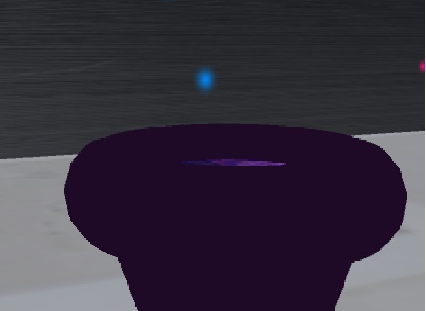
\includegraphics[scale=0.3]{Lucidite.png}

\quad

\textit {Figure 4 : Source de lucidité}

\end{center}

\quad

		\subsubsection{Ce qu'il reste à faire:}
\quad

Le travail qu'il me reste à faire pour les prochaines soutenances est assez considérable. Je compte m'occuper de la création des maps des niveaux 2 et 3, ainsi que de l'amélioration des textures. Je compte aussi créer des armes grâce à Blender que l'on pourra utiliser lors du jeu. Comme nous devons avoir le réseau pour la deuxième soutenance, je m'occuperai aussi de nous faire un joli personnage. De plus j'aiderai Thomas pour le moteur physique et j'assisterai Charles pour le Gameplay. 

\quad
\newpage

		\subsubsection{Conclusion personnelle:}

\quad

A la fin de cette première période, je pense que ce projet va nous apporter beaucoup de choses. A commencer par l’apprentissage du travail en groupe. Bien qu’il y ait une bonne cohésion dans notre groupe et que c’est sympa de travailler ensemble, parfois ce n’est forcément évident de réussir à mettre tout le monde d’accord. Il nous permet aussi d’enrichir nos connaissances.
Pour cette première soutenance, je ne pense pas avoir de retard par rapport au planning prévu.

\quad

\newpage

	\subsection{Thomas "Tetra" DELECROIX :}

\quad


		\subsubsection{ce qui a été fait :}

Pour la partie script voilà les principaux script que j’ai réalisé :

Deplacement/Camera : ce script, bien qu’il soit assez explicite, ne fut pas facile au début comme je venais de débuter sur Unity, il a fallu que je m’habitue à utiliser les fonctions de celui-ci. Ce script regroupe donc les fonctions permettant de déplacer et de pivoter le personnage. Pour les déplacements c’est assez simples, selon la touche appuyée on va changer les coordonnées du vecteur vitesse que l’on va appliquer à notre personnage à chaque image. Pour la rotation on va juste tourner le personnage en fonction d’un angle compris entre deux valeurs extrêmes permettant de limiter celui-ci.
Stuff : Ce script permet de stocker la lucidité qui va être représentée en pourcentage, et de l’exploiter avec des interactions d’objet. De base le personnage a un stock de lucidité de 100, celui-ci va diminuer si l’on ouvre une porte, ou projette des objets sur le décor, tout cela en fonction d’un coefficient qui permet de gérer manuellement la lucidité utilisée pour interagir avec ces objets. Si jamais la lucidité atteint 0, le niveau est remis à zéro pour ne pas rendre les énigmes trop faciles, le personnage meurt et réapparaît au dernier Checkpoint en faisant appel à un autre script. Pour contrer cela nous avons des sources de lucidité qui permettent de régénérer notre lucidité quand nous sommes proches d’elles. Pour projeter des objets sur le décor, nous avons un objet de base dont nous allons générer une nouvelle instance avec les coordonnées du personnage et son vecteur directeur de vision si le nombre de nouvelle instance déjà créé n’est pas élevée. Puis nous rajoutons un script pour que l’objet se comporte comme nous le souhaitions.
Porte : Ce script est assez simple et permet de gérer l’ouverture de la porte ainsi que la valeur de lucidité qu’il lui a été donnée.
Clip: Ce script est appliqué à l’objet instancié du script Stuff, on appellera cet objet Clip. Il permet dans ce cas d’avancer selon l’axe du regard du joueur tant que cet objet ne rencontre pas d’autre objet. Le but sera de lancer un Clip sur un mur et un autre sur une plate-forme amovible manuellement, cela va produire une attirance de la plate-forme par le clip collé sur le mur et donc déplacer la plate-forme vers ce mur tant que celle-ci ne rencontre pas le mur auquel elle s’est liée. Quand cela est fait les deux Clips vont se détruire pour un soucis de clarté de la map. Ils vont faire de même dans un autre cas pour compliquer un peu le jeu : si les clips ne sont pas attachés à un objet au bout de 5 secondes après leurs générations ils sont détruits, cela est la même chose s’ils sont attachés à un mur depuis plus de 5 secondes sans avoir eu de Clip attiré par eux-mêmes. Ce script va aussi gérer le fait que si un personnage se situe sur une plate-forme qu’il manipule, le personnage va rester sur celle ci.
Autop : Comme nous avons parlé de plates-formes amovibles manuellement, il y a aussi les plates-formes amovibles automatiquement. Ce script va gérer le déplacement de ce type de plates-formes qui va faire des simples allers retours entre les positions de départ et d'arrivée. Il va utiliser le même bout de script que pour les autres plates-formes pour gérer le cas du personnage qui est sur le plate-forme.



\quad

\begin{center}

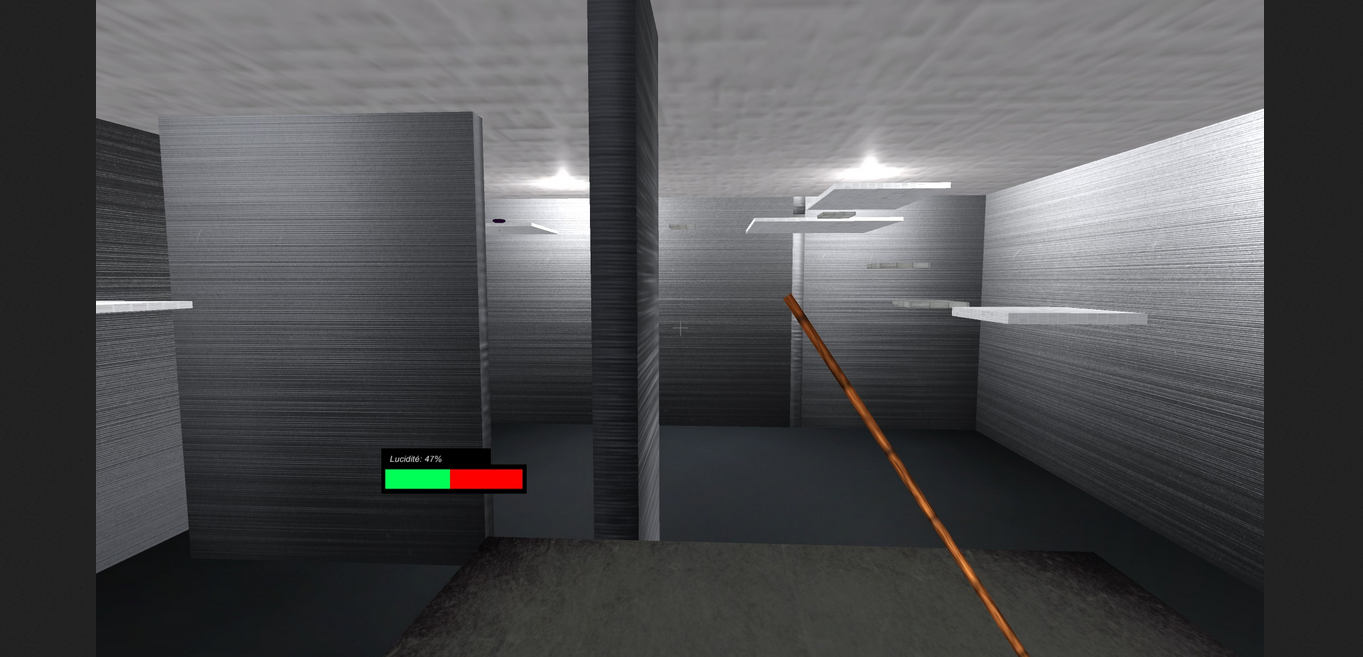
\includegraphics[scale=0.3]{Vue.png}

\quad

\textit {Figure 5 : Vue d'ensemble des plateformes}

\end{center}


\quad


		\subsubsection{Ce qu'il reste à faire:}

\quad

Je pense continuer à me concentrer sur la partie script et j’ai déjà pas mal d’idée concernant les prochaines mécaniques de jeu que je vais pouvoir développer. Pour la prochaine soutenance il va aussi nous falloir un réseau que je vais devoir créer.
\quad
		\subsubsection{Conclusion personnelle:}

\quad

Pour cette première soutenance je pense avoir pas mal développé ma connaissance et ma maîtrise des bases d’Unity. Grâce au travail de groupe j’ai également pu apprendre plus de chose même sur ce que je ne codais pas. Pour moi le projet est un peu plus avancé que ce que l’on avait prévu donc cela ne peux que nous motiver plus.

\quad
\newpage

	\subsection{Charles "Gigi" GINANE :}

\quad

		\subsubsection{ce qui a été fait :}

Durant les premiers jours du projet, j'ai appris les bases de Unity et j'ai réalisé quelques tutoriels.
Je me suis beaucoup familiarisé avec BitBucket et SourceTree afin de pouvoir travailler notre projet.

\underline{Gameplay} : j'ai géré une bonne partie du gameplay sur le projet.
Je me suis occupé de créer l'HUD ou l'ATH, c'est ce qui s'affiche sur l'écran du joueur en permanence.
L'HUD contient la barre de lucidité ressemblant à une barre de vie, le curseur, des textes qui s'affichent, etc.
L'HUD n'a pas été une tâche simple vu que le logiciel Unity était nouveau pour moi donc j'ai eu du mal à trouver ce que je souhaitais afin de réaliser l'HUD.
L'HUD a été fait avec des UI assez simples, j'ai utilisé des images pour réaliser la plupart de mon HUD, par exemple pour la barre de lucidité, j'ai utilisé 3 images, une pour faire le fond noir et les contours, une pour faire le fond rouge et une représentant la barre verte et en jouant sur l'échelle de X entre 0 et 1 on arrive à générer une barre de vie, de lucidité dans ce cas. Quelques scripts après, la barre de lucidité devient.
Le viseur n'est tout simplement que deux barres qui se croisent en leur milieu, une horizontale et une autre verticale.
Le bâton de bois est tout simplement un rectangle que j'ai customisé à l'aide d'une image de bois afin que la bâton soit le plus réaliste possible.
Enfin, les textes qui s'affichent nous expliquant les objets que l'on croise dans le jeu est un component qui modifie le texte qui se modifie à l'aide d'un script C\# que j'ai relié entre le code et l'UI.
Par exemple, dès que le joueur approche d’une source de lucidité , un message apparaît disant à quoi sert l’objet à proximité du joueur.
Je me suis occupé de réparer quelques problèmes liés au jeu et d’implémenter des scripts pour que le jeu puisse marcher intégralement pour cette soutenance.

    \underline{LaTeX} : Je suis aussi le gérant LaTeX du groupe, c'est-à-dire que je m'occupe de mettre en forme tous les documents que nous devons fournir lors de ce projet en LaTeX. Cela présente un avantage car nous n'avons pas besoin de perdre du temps à apprendre le LaTeX.

Les difficultés que j’ai rencontrées portent principalement sur l’utilisation de Unity étant donné que c’était un nouvel univers auquel j’étais confronté et la manipulation de ce dernier n’a pas été de tout repos . L’utilisation de Git a été difficile à prendre en main mais révèle de nombreux avantages en ce qui concerne le travail de groupe. 


\newpage 

\begin{center}

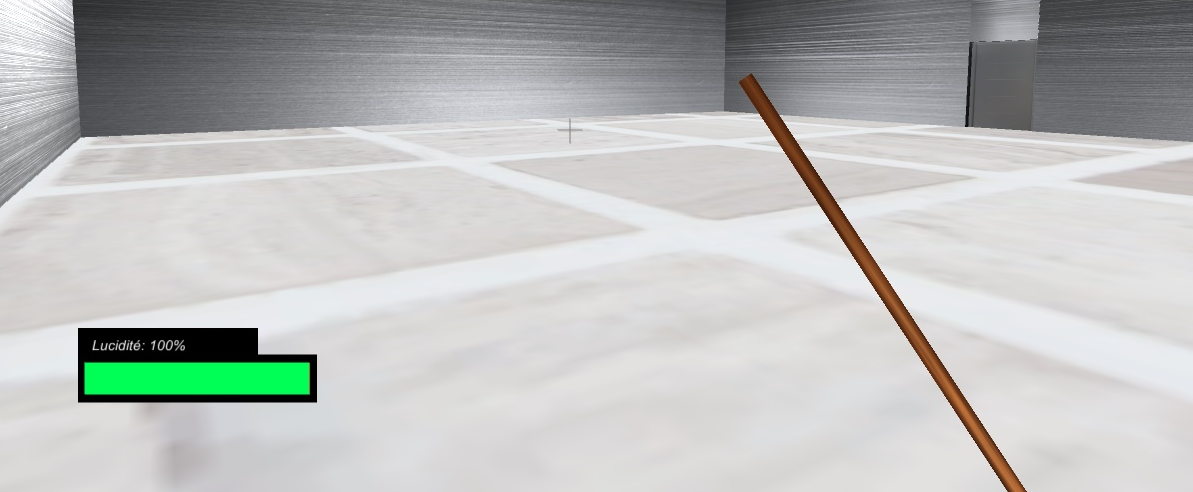
\includegraphics[scale=0.55]{HUD.png}

\quad

\textit {Figure 6 : HUD}

\end{center}


\quad

		\subsubsection{Ce qu'il reste à faire:}

\quad

Le travail à fournir est tout de même conséquent, maintenant que nous possédons les bases sur notre jeu, nous allons nous en servir pour améliorer le projet.
Je vais me consacrer à améliorer l’HUD pour qu’il soit plus en rapport avec le thème du jeu et modéliser les armes qui seront disponibles ultérieurement pour que le joueur puisse savoir quelle arme il a en main. j’aiderai Laurent à continuer d’implémenter les sons dans le jeu et voire, d’ajouter une musique aux différents niveaux et au menu.
Je m’occuperai aussi de la gestion du site du projet pour les modifications futures afin qu’il soit le plus complet possible.
J’améliorerai aussi le gameplay en créant de nouveau élément dans l’HUD et au sein du jeu.

\quad
\newpage

		\subsubsection{Conclusion personnelle:}


\quad

Au terme de cette première période, à savoir de la validation du cahier des charges jusqu'à la première soutenance, j'ai un bon ressenti de ce que j'ai pu réaliser par rapport à mes capacités mais aussi par ce que le groupe à pu fournir pour cette première soutenance.
Je pense avoir pas mal apporté de mes connaissances aux groupes mais aussi, j'ai pu enrichir mes connaissances en code grâce à mes camarades.
Nous avons une bonne cohésion de groupe, on est tous complémentaires et cela nous permet de bien avancer.
Je ne me sens pas en retard par rapport à ce que j’avais prévu de faire dans le cahier des charges pour la première soutenance.
Je suis très confiant face à la suite de notre projet vu que nous avons réalisé la majorité des bases pour notre jeu donc il ne nous reste plus qu’à continuer dans notre bonne lancée afin de pourvoir réaliser notre projet à bien.

\quad
\newpage

	\subsection{Laurent "Aluxima" MARCHAUD:}


\quad

		\subsubsection{ce qui a été fait :}

\quad

La construction du site a été mon travail le plus conséquent pour cette première phase. Je m’y suis pris très tôt, et il a très rapidement été opérationnel. J’avais déjà acqui des bases en html/php/css en terminale en I.S.N. et pendant mon temps libre. Il a fallu que j’apprenne à utiliser une base de données MySQL et l’utiliser dans du code php. C’est une chose qui m’intéressait depuis longtemps mais je n’étais jamais allé plus loin pour apprendre.
Le site est hébergé actuellement sur mon Raspberry Pi, mais ma ligne ADSL ayant été endommagée quelques jours avant la soutenance, il a fallu le déménager chez Thomas pour que le site soit accessible depuis l’extérieur.

    Le plus difficile a été d’apprendre à utiliser Unity, et à bien l’utiliser. A premier abord, on se retrouve dans une interface graphique complexe avec plein d’onglets, de menus, d’options, de choses à glisser, etc. Mais dès que l’on a regardé quelques vidéos d’apprentissage du logiciel, on s’y retrouve rapidement et on se repère très vite. Je pense que la maîtrise de Unity est proportionnelle au temps que l’on passe dessus. Il y a toujours des choses à apprendre. 
La plus grande aide est Google. Dès que l’on rencontre un problème dans le logiciel ou que l’on ne sait pas faire quelque chose, il suffit de chercher sur Google et on trouve instantanément des réponses dans des forums, des vidéos, des manuels…

    Mes contributions au développement du jeu pour cette première phase ont été principalement la gestion de tous les menus présents dans le jeu et leurs interactions, la gestion des “checkpoints”, les particules de la source de lucidité, et l’ajout de sons.
Les menus sont les suivants: 
Une scène isolée du menu principal avec un bouton lançant le mode solo, un bouton du mode multijoueur (inactif pour l’instant), un bouton ouvrant le menu d’options, et un bouton pour quitter le jeu.
Un menu pause qui s’affiche quand on appuie sur la touche “échap”, qui affiche un bouton lançant le menu d’options, un bouton pour reprendre le jeu, et un pour revenir au menu principal.
Pour l’instant, le menu d’options est inutile car les réglages présents (volume sonore et sensibilité de la souris) sont inactifs.
Les checkpoints comprennent l’endroit où le personnage apparaît au début, les points que le personnage peut acquérir et réapparaître dessus quand il meurt, les zones où le personnage est censé mourir, et le point final, affichant un menu de fin du niveau. Le checkpoint actuel sur lequel le personnage est censé réapparaître quand il meurt est stocké dans une variable qui change quand il en rencontre un autre.
Les sons ne sont encore que des tests. La source de lucidité émet un bruit lorsque l’on s’en rapproche et le jeu joue un son lorsque le personnage meurt.

\quad

\begin{center}

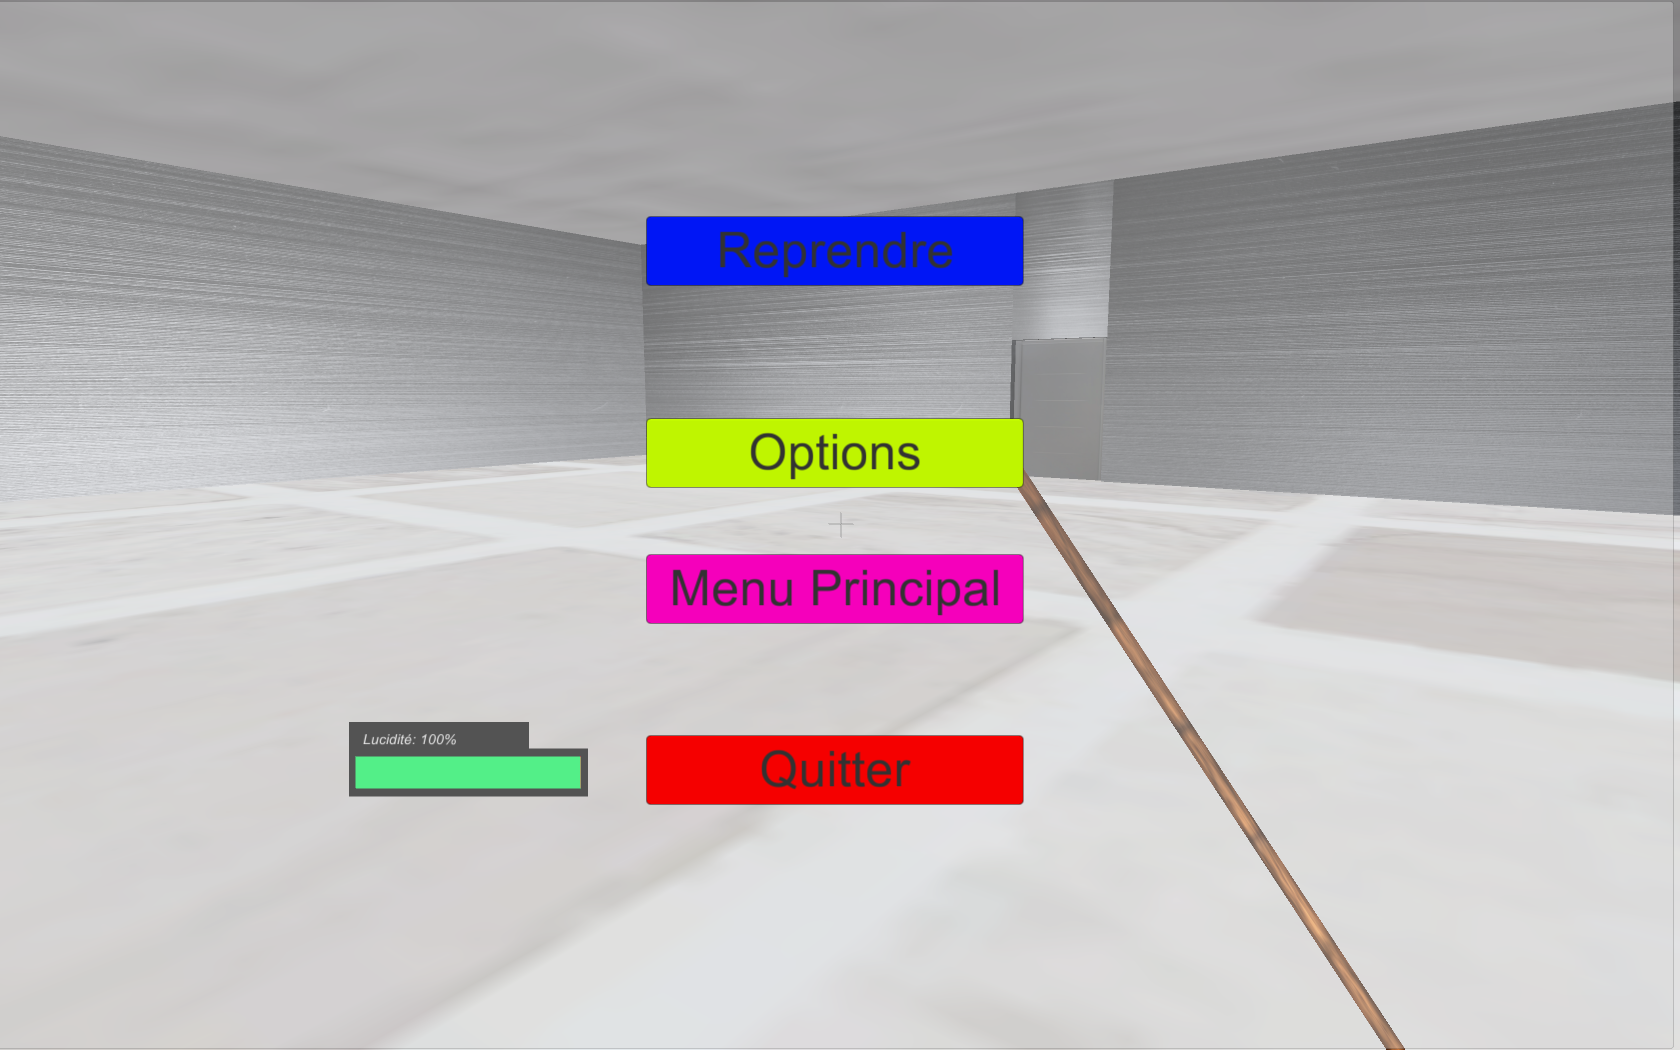
\includegraphics[scale=0.27]{Menu.png}

\quad

\textit {Figure 7 : Le menu pause }

\end{center}



\quad

\begin{center}

\includegraphics[scale=0.27]{Reglages.png}

\quad

\textit {Figure 8 : Le menu des réglages}

\end{center}


\quad

		\subsubsection{Ce qu'il reste à faire:}

\quad

    Le site web reste à terminer puisqu’il nous faudrait un moyen de supprimer et modifier les news sans exécuter des resquêtes SQL en passant par le ssh du Raspberry Pi.
Les sons du jeu sont à refaire car il serait beaucoup plus pratique de créer un gestionnaire de sons qui gérerait tous les sons du jeu. Ainsi, il sera facile de tous les mettre en pause, modifier leurs volumes, etc.
Il reste encore toute la partie multijoueur à faire avec Thomas et je suis conscient que cela nécessitera beaucoup de travail car il faudra quasiment tout reprendre.
D’autres interactions du personnage sont à créer. Je suis en train de faire une corde sur laquelle on se balancerait, ou qui pourra être lancée comme un grapin, il faudra voir ce qui va le mieux.
Pour le moment, notre personnage est représenté par une simple capsule, mais il faudra créer un vrai personnage.

\quad

		\subsubsection{Conclusion personnelle:}

\quad

En cette courte période, j’ai beaucoup appris, que ce soit en code (requêtes SQL, PHP, C\#), ou dans l’utilisation de Unity. 
Ce projet me motive énormément. Dès que je commence quelque chose, je n’arrive pas à m’arrêter tant que je ne l’ai pas terminé.
Les délais que nous nous étions imposés sont respectés et notre rythme est bon dans le groupe.

\quad

\newpage


\section {Le site WEB}

\quad

    Le site web lucidity.aluxima.ovh est bien plus avancé que ce que l’on avait prévu pour la première soutenance. En effet, on peut dire que ce dernier est presque achevé. C’est l’un des éléments du projet commencés en premier. Il permet aux visiteurs d’accéder à 6 pages principales:

 - La page d’accueil, avec une brève présentation du site ainsi que le logo du groupe “The Chamallow”
 - La page des news, sur laquelle sont affichés les actualités d’avancement du projet, les impressions des membres du groupe et tout ce que l’on veut écrire dessus. Chaque membre a donc la possibilité de rajouter des nouvelles.
 - Une page de présentation du groupe, la même que celle présente dans le cahier des charges. Elle contient une brève présentation du groupe en général, et les présentations individuelles.
 - Une page de téléchargements, sur laquelle l’utilisateur peut télécharger différents éléments comme les documents (Cahier des charges, rapports de soutenance…) et la dernière version du jeu, si l’utilisateur est connecté.
 - Une page de contact, contenant nos adresses email EPITA sur lesquelles on peut nous contacter.
 - Une dernière page d’utilisateur. Si l’utilisateur n’est pas connecté, cette dernière est une page de connexion avec deux champs: login et mot de passe. Un bouton redirigeant vers une page d’enregistrement où l’utilisateur peut créer un compte en entrant un login et en répétant un mot de passe.

\quad

\quad

\begin{center}

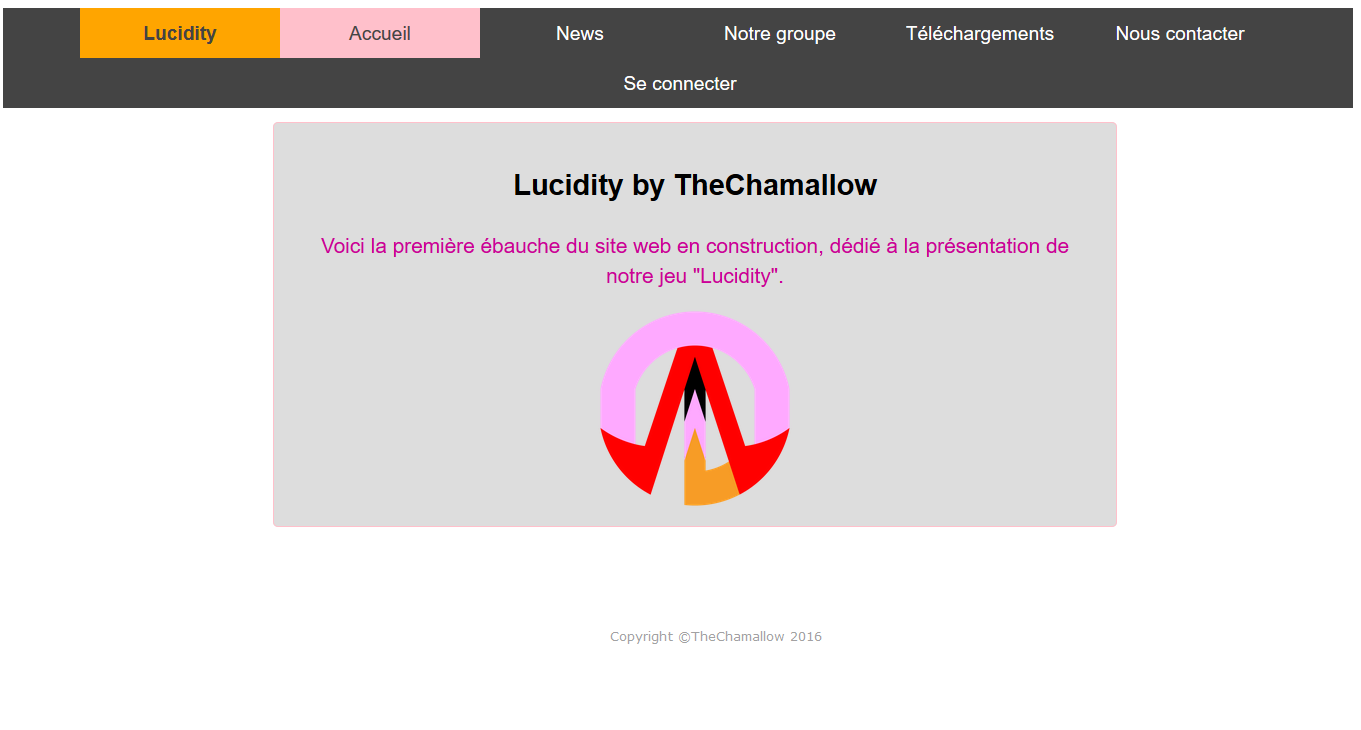
\includegraphics[scale=0.35]{Site.png}

\quad

\textit {Figure 9 : Page d'accueil du site }

\end{center}


\quad

\newpage

Si l’utilisateur est connecté, il verra sur sa page personnelle un bouton redirigeant vers une page lui permettant de modifier son mot de passe.
Le menu déroulant sous l’onglet de la page utilisateur  s’adapte à l’authentification ou non de l’utilisateur: S’il est connecté, le menu affiche un bouton de déconnexion. Sinon, il affiche un menu de connexion et un bouton redirigeant vers la page de création d’un compte.

Ce site web est pour l’instant hébergé chez l’un des membres sur un Raspberry Pi utilisant Apache et MySQL. Il sera certainement hébergé dans le futur sur une plateforme d’hébergement dédiée et un nom de domaine avec le nom du jeu sera pris
.
Son développement a été fait depuis rien. Aucun modèle de site web n’a été copié. Il a d’abord fallu créer la structure générale des pages en html et css puis les éléments dynamiques comme les news et la gestion des utilisateurs ont été ajoutés en php en utilisant une base de données MySQL.

Les utilisateurs sont enregistrés dans une table de données contenant les éléments login, mot de passe crypté en MD5 (bien que obsolète) et un entier permissions. Les permissions correspondent à un rang. Plus l’utilisateur a un rang haut, plus il a de droits. Ainsi, un utilisateur de base a un rang de 1 lui permettant d’accéder au lieu de téléchargement de la dernière version du jeu, et les membres du groupe ont un rang de 10 leur permettant d’ajouter des news.

Les news sont aussi enregistrées dans une table de données, contenant les champs id (entier incrémenté automatiquement), contenu de la news, titre, date, et auteur.

Les améliorations que l’on pourrait apporter au site seraient les suivantes:

Ajouter aux membres du groupe des options de suppression et de modification des news.

Un meilleur chiffrement des mots de passe des utilisateurs dans la base de données.

Une meilleure présentation du projet sur la page d’accueil


D’autre part, il serait intéressant pour le futur d’utiliser la base de données des utilisateurs pour la connexion au mode multijoueur dans le jeu, le stockage de la progression des joueurs, etc.

\quad

\newpage

\section{conclusion}

\quad

    Pour conclure, nous sommes plutôt satisfaits de ce que nous avons fait puisque tous nos objectifs pour la première soutenance ont été remplis avec succès. De plus, nous avons un peu d’avance en ce qui concerne le site, la physique et le gameplay. Pour la prochaine soutenance, il ne nous reste plus qu’à continuer sur notre lancée.

\quad

\quad

\begin{center}

\textbf{The Chamallow !!!!}

\end{center}








\end{document}